\section{Background on \texorpdfstring{$\mathrm{Cl}(3,0)$}{Cl(3,0)} and the geometric product}\label{supp:prelim}

The real Clifford algebra $\mathrm{Cl}(3,0)$ is the eight-dimensional associative unital algebra generated by an orthonormal basis $\{e_1, e_2, e_3\}$ of $\mathbb{R}^3$ subject to $e_ie_j + e_je_i = 2\delta_{ij}$ \citep{lounesto2001clifford}. A basis of $\mathrm{Cl}(3,0)$ ordered by grade is $\{1,\; e_1, e_2, e_3,\; e_{12}, e_{13}, e_{23},\; e_{123}\}$, corresponding respectively to a scalar (grade 0), three vectors (grade 1), three bivectors (grade 2), and a pseudoscalar (grade 3), so any multivector $X \in \mathrm{Cl}(3,0)$ has a unique grade decomposition $X = X^{(0)} + X^{(1)} + X^{(2)} + X^{(3)}$ \citep{ruhe2023gcan}.

The geometric product is the bilinear, associative, unital extension of the generator relations, with the vector decomposition \citep{brandstetter2022clifford} below: for two vectors $u, v \in \mathbb{R}^3$ embedded in $\mathrm{Cl}(3,0)$ it decomposes as $uv = u \cdot v + u \wedge v$, where $u \cdot v = \tfrac{1}{2}(uv + vu) = \sum_i u_iv_i$ is the symmetric scalar part and $u \wedge v = \tfrac{1}{2}(uv - vu) = \sum_{i<j}(u_iv_j - u_jv_i)e_{ij}$ is the antisymmetric bivector part.

With $I=e_1e_2e_3$, $I^2=-1$ and $I^{-1}=-I$, we adopt the bivector dual convention $\star\alpha=\alpha I^{-1}$ \citep{doran2003geometric}. Direct computation yields the sign convention
\[
\star e_{12} = +e_3,\qquad \star e_{13} = -e_2,\qquad \star e_{23} = +e_1,
\]
which gives $\star(u\wedge v)=u\times v$ by substitution. The dual is rotationally equivariant, but its vector output is axial: under inversion, $e_ie_j \to (-e_i)(-e_j)=e_ie_j$, giving parity $+1$ rather than the polar-vector parity $-1$ \citep{geiger2022e3nn}. We apply this distinction to the readout in Section~\ref{supp:so3_o3}.

The geometric product is $\mathrm{SO}(3)$-equivariant under the rotor action: for any rotor $R = \exp(-\theta B/2)$ built from a unit bivector $B$ and any multivectors $a, b$, conjugation $a \mapsto RaR^{-1}$ preserves the product, $R(ab)R^{-1} = (RaR^{-1})(RbR^{-1})$ \citep{ruhe2023cgenn}. This product-preserving action underlies the Clifford track.

\section{Architectural comparison with ICTP}\label{supp:ictp}

ICTP builds an $\mathrm{O}(3)$-equivariant architecture from irreducible Cartesian tensors, combines ranks through irreducible tensor products, and constructs higher-body-order features through repeated products \citep{zaverkin2024ictp}. CliffordSTF shares the STF foundation but retains a parallel Clifford substrate; the following four points specify our design choices.

\textbf{Algebraic substrate.} CliffordSTF runs a Clifford $\mathrm{Cl}(3,0)$ multivector track in parallel with the STF tracks, and the Clifford track carries both scalars and pseudoscalars that have a natural parity structure through the grade involution, as well as bivectors that expose an extra $L{=}1$ axial channel via the Hodge star. The STF tracks in CliffordSTF supply the $L{=}2$ and $L{=}3$ components that the Clifford geometric product cannot reach, not the entire equivariant substrate.

\textbf{Bilinear operation.} CliffordSTF uses two different bilinears in tandem: the Clifford geometric product acting on the 8-dimensional multivector via an $8 \times 8$ Cayley table, and a small set of closed-form symmetric-traceless contractions acting on the STF tracks. The Clifford product handles scalar, vector, bivector, and pseudoscalar channels with a single contraction; the STF operations handle rank-2 and rank-3 tensors through explicit symmetrisation and trace removal. The two are coupled bijectively to Clebsch--Gordan channels as specified in Theorem~\ref{M-thm:cg_completeness} and its higher-order extensions.

\textbf{Cross-track coupling.} In CliffordSTF the Clifford and STF tracks are coupled bidirectionally: the STF$_2$ track is generated from grade-1 vector features via $\mathrm{STF}_2(\hat{r}_{ij}, h_j^{\mathrm{vec}})$, and is fed back into the grade-1 vector component of the Clifford message through the $S \cdot v$ contraction. The \texttt{stf2\_no\_cross} variant does not regress relative to the CliffordIP base: it reaches $f_{cos}{=}0.456$ and $e_{\mathrm{MAE}}{=}25.8$\,meV against $0.030$ and $125.8$\,meV for vanilla $L{=}1$ Clifford (Table~\ref{tab:ablation_full}), because the $L{=}2$ edge descriptor supplies angular content to message passing whether or not the tracks are coupled. The full STF$_2$+STF$_3$ configuration has one fewer divergent run with coupling and a lower median energy MAE in this sample; paired statistics are reported in Section~\ref{supp:cross_stability}.

\textbf{Equivariance scope.} CliffordSTF proves $\mathrm{SO}(3)$ equivariance; under $\mathrm{O}(3)$, the polar-vector grade-1 component and the axial-vector Hodge-of-bivector component would need distinct parity labels $1^-$ and $1^+$ respectively (Section~\ref{M-sec:readout}, Section~\ref{supp:so3_o3}). The current implementation concatenates the two in the force readout under the $\mathrm{SO}(3)$ framework, which is consistent under rotations but would need refactoring for full $\mathrm{O}(3)$.

CliffordSTF retains geometric-product message passing while adding STF features through explicit cross-track maps. The ablation in Section~\ref{M-sec:ablation} evaluates the contribution of each component.

\section{Rotational content of projective multivectors}\label{supp:gatr}

GATr \citep{brehmer2023geometric} uses the 16-dimensional projective algebra $\mathrm{Cl}(3,0,1)$. Applying the rotation action to its basis, the null basis vector is unchanged; the decomposition of main-text eqn~(\ref{M-eq:cl_irreps}) therefore occurs twice, giving $4\cdot(L{=}0)\oplus4\cdot(L{=}1)$. Thus neither multivector representation contains an explicit $L{\geq}2$ irrep. This statement concerns the representation carried by the multivector, rather than the expressivity of a complete nonlinear network.

\section{\texorpdfstring{$\mathrm{SO}(3)$}{SO(3)} versus \texorpdfstring{$\mathrm{O}(3)$}{O(3)} equivariance}\label{supp:so3_o3}

All guarantees stated in \S\ref{M-sec:method} are $\mathrm{SO}(3)$-equivariance guarantees. Polar and axial vectors carry equivalent $L{=}1$ representations under $\mathrm{SO}(3)$, but differ by a factor of $\det(R)$ under $R\in\mathrm{O}(3)$, following the parity convention used in \texttt{e3nn} \citep{geiger2022e3nn}. Consequently, our rotational readout can concatenate them, while reflection-equivariant mixing would require the distinct labels in Table~\ref{tab:parity}.

\begin{table}[!htbp]
\centering
\caption{$\mathrm{O}(3)$ parity labels for the tracks used in CliffordSTF. The general rule is $\mathrm{STF}_\ell$ built from polar vectors has parity $(-1)^\ell$, matching the parity of the spherical harmonic $Y_{\ell m}(-\hat{n}) = (-1)^\ell Y_{\ell m}(\hat{n})$ \citep{varshalovich1988quantum}.}\label{tab:parity}
\small
\begin{tabular}{lccc}
\toprule
Object & Physics analog & Parity & $\mathrm{O}(3)$ label \\
\midrule
Grade-0 scalar & charge $q$ & $+$ & $0^+$ \\
Grade-1 vector $e_i$ & position $\mathbf{r}$ & $-$ & $1^-$ (polar) \\
Grade-2 bivector $e_{ij}$ / Hodge dual & angular momentum $\mathbf{L}{=}\mathbf{r}\times\mathbf{p}$ & $+$ & $1^+$ (axial) \\
Grade-3 pseudoscalar $I$ & triple product $\mathbf{a}\cdot(\mathbf{b}\times\mathbf{c})$ & $-$ & $0^-$ \\
$\mathrm{STF}_2$ from polar vectors & quadrupole $Q_{ij}$ & $+$ & $2^+$ \\
$\mathrm{STF}_3$ from polar vectors & octupole $O_{ijk}$ & $-$ & $3^-$ \\
\bottomrule
\end{tabular}
\end{table}

Extending our model to full $\mathrm{O}(3)$ equivariance would require distinguishing the $1^-$, $1^+$, $2^+$ and $3^-$ tracks and using parity-compatible mixing and readout, following the parity-aware tensor-product construction used in ICTP \citep{zaverkin2024ictp}.

\section{Derivation of the STF coefficients}\label{supp:stf_coefficients}

We work through the classical STF projection \citep{coope1965irreducible} to recover the three rational coefficients used in \S\ref{M-sec:stf_channels}.

\textbf{STF$_2$ detracing coefficient $\tfrac{1}{3}$.} In $d$ dimensions, the symmetric traceless part of a rank-2 tensor requires subtracting $\tfrac{1}{d} \delta_{ij} T_{kk}$ to enforce $\sum_i T_{ii}^{\text{sym-traceless}} = 0$ \citep{stone2013theory}. Direct check in $d=3$: $\delta_{ii} \mathrm{STF}_2(u,v)_{ii} = (u\cdot v) - \tfrac{1}{3}(3)(u\cdot v) = 0$.

\textbf{STF$_3$ trace vector coefficient $\tfrac{2}{3}$.} Since $S_{ij}$ is symmetric traceless ($S_{ii}=0$), the trace of $T^{\text{sym}}_{ijk}$ over any pair of indices reduces to two of the three summands:
\[
T^{\text{sym}}_{iik} = \tfrac{1}{3}(S_{ii}v_k + S_{ik}v_i + S_{ik}v_i) = \tfrac{1}{3}(0 + 2\,S_{kl}v_l) = \tfrac{2}{3}\,S_{kl}v_l.
\]
By full symmetry, $T^{\text{sym}}_{iki} = T^{\text{sym}}_{kii} = A_k$ as well.

\textbf{STF$_3$ detracing coefficient $\tfrac{1}{5}$.} Set $U_{ijk} = T^{\text{sym}}_{ijk} - \alpha(\delta_{ij}A_k + \delta_{ik}A_j + \delta_{jk}A_i)$ and require $U_{iik} = 0$. Computing the trace:
\[
U_{iik} = A_k - \alpha(3A_k + A_k + A_k) = A_k - 5\alpha A_k \implies \alpha = \tfrac{1}{5}.
\]
More generally, the three-dimensional per-delta first-trace coefficient at rank $\ell$ is $1/(2\ell - 1)$, yielding $\tfrac{1}{3}$ at $\ell{=}2$, $\tfrac{1}{5}$ at $\ell{=}3$, $\tfrac{1}{7}$ at $\ell{=}4$ \citep{thorne1980multipole}. Applequist gives the fully detraced closed form for arbitrary rank \citep{applequist1989traceless}.

\textbf{Degrees-of-freedom check for STF$_3$.} The symmetric rank-3 tensor $T^{\text{sym}}$ in $\mathbb{R}^3$ has $\binom{3+3-1}{3} = 10$ independent components; subtracting the 3-component trace vector $A$ leaves $10 - 3 = 7 = 2\ell + 1$ for $\ell = 3$, matching the dimension of the $L{=}3$ irrep of $\mathrm{SO}(3)$ \citep{shao2025orthonormal}.

\section{Explicit coordinate formulas for the constructive CG maps}\label{supp:cg_proof}

We enumerate every constructive map used in the architecture and verified in Section~\ref{supp:cg_test}. The formulas use classical irreducible Cartesian tensor coupling \citep{coope1965irreducible} and the STF coefficients derived in Section~\ref{supp:stf_coefficients}.

\textbf{$\mathbf{1} \otimes \mathbf{1} \to \mathbf{0} \oplus \mathbf{1} \oplus \mathbf{2}$.} For $u, v \in \mathbb{R}^3$:
\begin{itemize}
    \item $L{=}0$: $(u \otimes v)_{L=0} = u \cdot v = u_iv_i$.
    \item $L{=}1$: $(u \otimes v)_{L=1} = \star(u \wedge v)_i = \varepsilon_{ijk}u_jv_k$, equivalently the cross product $u \times v$.
    \item $L{=}2$: $(u \otimes v)_{L=2} = \mathrm{STF}_2(u,v)_{ij} = \tfrac{1}{2}(u_iv_j + u_jv_i) - \tfrac{1}{3}(u\cdot v)\delta_{ij}$.
\end{itemize}

\textbf{$\mathbf{2} \otimes \mathbf{1} \to \mathbf{1} \oplus \mathbf{2} \oplus \mathbf{3}$.} For a symmetric traceless $S \in \mathbb{R}^{3\times 3}$ and $v \in \mathbb{R}^3$:
\begin{itemize}
    \item $L{=}1$: $(S \cdot v)_i = S_{ij}v_j$.
    \item $L{=}2$: symmetric traceless part of $\varepsilon_{ikl}S_{jl}v_k$, i.e.\ $[\mathrm{sym}(S\times v) - \tfrac{1}{3}\mathrm{tr}(\cdot)\mathbb{I}]$; explicit 5-component formulas are in the code release (\texttt{contract\_stf2\_vec\_to\_stf2}).
    \item $L{=}3$: $\mathrm{STF}_3(S, v)_{ijk} = S_{(ij}v_{k)} - \tfrac{1}{5}(\delta_{ij}A_k + \delta_{ik}A_j + \delta_{jk}A_i)$ with $A_k = \tfrac{2}{3}S_{kl}v_l$; the coefficients $\tfrac{2}{3}$ and $\tfrac{1}{5}$ follow from the trace calculations in Section~\ref{supp:stf_coefficients}.
\end{itemize}

\textbf{$\mathbf{2} \otimes \mathbf{2} \to \mathbf{0} \oplus \mathbf{1} \oplus \mathbf{2} \oplus \mathbf{3}$ (with $L{=}4$ omitted).} For symmetric traceless $S_1, S_2$:
\begin{itemize}
    \item $L{=}0$: $\langle S_1, S_2 \rangle_F = S_{1,ij}S_{2,ij}$ (Frobenius inner product).
    \item $L{=}1$: antisymmetric contraction $\varepsilon_{ijk}S_{1,jl}S_{2,kl}$.
    \item $L{=}2$: symmetric traceless projection of $S_{1,ik}S_{2,kj}$.
    \item $L{=}3$: an analogous symmetric-then-detraced construction treating one operand as a vector-indexed rank-2 tensor.
    \item $L{=}4$: outside our $L_{\max}{=}3$ cut and not used.
\end{itemize}

\textbf{$\mathbf{3} \otimes \mathbf{1} \to \mathbf{2} \oplus \mathbf{3}$ (with $L{=}4$ omitted).} For a symmetric traceless rank-3 tensor $T$ and vector $v$:
\begin{itemize}
    \item $L{=}2$: $(T \cdot v)_{ij} = T_{ijk}v_k$ followed by trace removal (\texttt{contract\_stf3\_vec\_to\_stf2}).
    \item $L{=}3$: analogous symmetric-then-detraced construction.
    \item $L{=}4$: omitted.
\end{itemize}

Each map is a polynomial in its inputs with constant rational coefficients. There are no learned Clebsch--Gordan coefficients, no Wigner-$D$ tables, and no calls to \texttt{e3nn} \citep{geiger2022e3nn}. All tensor products of $\mathrm{SO}(3)$ irreps above are multiplicity-free, consistent with the general $\mathrm{SU}(2)$ fact that $L_1 \otimes L_2 = \bigoplus_{L=|L_1-L_2|}^{L_1+L_2} L$ each with multiplicity one \citep{varshalovich1988quantum}.

\section{Numerical verification of the constructive CG maps and end-to-end equivariance}\label{supp:cg_test}

\textbf{Primitive-level verification.} The released tests compare the rank-2 and rank-3 STF products with explicit Cartesian symmetrisation and trace removal on $10^3$ random double-precision inputs. They also check that these products commute with proper rotations, using an absolute tolerance of $10^{-11}$. Separate checks cover geometric-product rotation covariance, grade-norm invariance and reverse involution. These checks test the implemented Cartesian identities; they do not constitute a comparison of every admissible coupling with Wigner $3j$-symbols.

\textbf{End-to-end checks.} The released tests apply a proper rotation and translation to a non-collinear molecular geometry, rebuild its radius graph, and compare energies and rotated forces at absolute tolerance $10^{-3}$ for the twelve ablation settings. They also test atom-permutation symmetry. For the energy-gradient model, finite-difference checks compare forces with $-\partial E/\partial x$ and test zero net force and torque. The tests are available in \texttt{tests/test\_physics.py} and \texttt{tests/test\_models\_algebra.py}.

\section{Edge embedding}\label{supp:edge_embed}

We expand pairwise distances $d_{ij} = \lVert\mathbf{r}_{ij}\rVert$ through Gaussian radial basis functions (RBFs), as in SchNet \citep{schutt2017schnet}, with centres evenly spaced between 0 and our cutoff $r_c$, and apply the cosine envelope $\phi_c(d_{ij}) = \tfrac{1}{2}[\cos(\pi d_{ij}/r_c) + 1]$ that drives edge features smoothly to zero at the cutoff. Two small MLPs map the RBF expansion to channel-wise scalar weights for the grade-0 part and channel-wise weights for the grade-1 part of the edge multivector; the grade-1 direction $\hat{r}_{ij}$ is then multiplied by the channel weights and placed in the vector component. For CliffordSTF variants with $\mathrm{stf\_mode} \neq \text{none}$, a third MLP produces channel weights for the STF$_2$ edge feature, populated with $\mathrm{STF}_2(\hat{r}_{ij}, \hat{r}_{ij})$ (a canonical $L{=}2$ descriptor of the edge direction). When $\mathrm{stf\_mode}=\text{stf2+stf3}$, the STF$_3$ edge block is initialised to zero and is populated only via message passing within node features.

\section{Augmented product at the many-body stage}\label{supp:aug_prod}

At the many-body stage of each interaction layer, an augmented product couples the Clifford and STF tracks through six bilinear terms. Given operands $a$ and $b$ each carrying Clifford, STF$_2$, and (optionally) STF$_3$ components, the augmented product computes:
\begin{itemize}
    \item The ordinary geometric product $a^{\mathrm{Cl}} b^{\mathrm{Cl}}$ via the $8\times8$ Cayley table;
    \item A new STF$_2$ from the grade-1 components via $\mathrm{STF}_2(a^{\mathrm{vec}}, b^{\mathrm{vec}})$;
    \item An updated STF$_2$ via the $L{=}2 \otimes L{=}1 \to L{=}2$ path, applied from either operand (symmetrised-then-detraced cross-contraction of $a^{\mathrm{STF}_2}$ with $b^{\mathrm{vec}}$, and vice versa);
    \item An $L{=}0$ contribution to grade-0 via $\langle a^{\mathrm{STF}_2}, b^{\mathrm{STF}_2}\rangle_F = a_{ij}^{\mathrm{STF}_2} b_{ij}^{\mathrm{STF}_2}$;
    \item A new STF$_3$ via $\mathrm{STF}_3(a^{\mathrm{STF}_2}, b^{\mathrm{vec}})$;
    \item An STF$_2$ update via $\mathrm{STF}_3 \otimes L{=}1 \to L{=}2$ contraction of $a^{\mathrm{STF}_3}$ against $b^{\mathrm{vec}}$.
\end{itemize}
Each term corresponds to a CG channel in one of the decompositions $\mathbf{1}\otimes\mathbf{1}$, $\mathbf{2}\otimes\mathbf{1}$, $\mathbf{2}\otimes\mathbf{2}$, or $\mathbf{3}\otimes\mathbf{1}$ enumerated in Section~\ref{supp:cg_proof}. These bilinears provide gradient paths between the Clifford and STF tracks. Their empirical effects are assessed in Section~\ref{M-sec:ablation} and Section~\ref{supp:cross_stability}.

\section{Equivariant normalisation and gating}\label{supp:normalization}

Each CliffordSTFLinear layer is block-diagonal across tracks: it applies independent linear maps of shape $C_{\mathrm{in}} \to C_{\mathrm{out}}$ over channels within the Clifford multivector, the STF$_2$ tensor, and the STF$_3$ tensor, without mixing them linearly. Cross-track information flow occurs only through the bilinear products described in \S\ref{M-sec:architecture}.

Track-wise equivariant normalisation rescales each track by a per-channel invariant norm. For the Clifford track we compute the squared per-grade Clifford norm $\lVert h^{(k)}\rVert^2$ as the scalar part of $h^{(k)}\widetilde{h^{(k)}}$, where $\widetilde{\cdot}$ is the reverse \citep{doran2003geometric}; for STF$_2$ we use the Frobenius norm $\lVert S\rVert_F^2 = S_{ij}S_{ij}$ with $S_{zz} = -S_{xx}-S_{yy}$ substituted; for STF$_3$ we use the analogous Frobenius norm with multiplicity factors reflecting the symmetric tensor structure. These scalar contractions are rotationally invariant, as required for equivariant norm-based nonlinearities \citep{ruhe2023cgenn,zaverkin2024ictp}.

Our activation applies SiLU \citep{elfwing2018silu} to grade-0 features and a sigmoid-gated rescaling to each $L \geq 1$ track: for a feature $f$ at rank $\ell \geq 1$, we compute $g = \sigma(\mathrm{MLP}(\lVert f\rVert))$ with the sigmoid MLP acting on the invariant norm, and output $g \cdot f$. Multiplication by an invariant scalar gate preserves equivariance, following the gating constructions of \citet{weiler20183d,schutt2021painn}; we apply this principle separately to the three tracks.

\section{Adaptive \texorpdfstring{$L$}{L}-track routing}\label{supp:routing}

Our adaptive routing modulates the STF tracks using invariant gates. It is applied as a per-atom, per-track multiplicative gate $g_\ell \in [0, 1]$ between message-passing layers, rescaling the STF$_\ell$ track as $h^{\mathrm{STF}_\ell}_i \leftarrow g_\ell^{(i)} \cdot h^{\mathrm{STF}_\ell}_i$. The Clifford track is always active. Three modes are supported.
\begin{itemize}
    \item \textbf{None.} All atoms use all tracks; $g_\ell^{(i)} = 1$.
    \item \textbf{Static.} Gates are learned per atomic type via a small embedding table.
    \item \textbf{Learned.} Gates are produced by a two-layer MLP with sigmoid output applied to four per-atom invariant descriptors: (i) coordination number $|\mathcal{N}(i)|$, (ii) angular variance $1 - \lVert\bar{r}_i\rVert$ where $\bar{r}_i = \tfrac{1}{|\mathcal{N}(i)|}\sum_{j\in\mathcal{N}(i)}\hat{r}_{ij}$, (iii) mean neighbour distance, (iv) grade-0 feature norm averaged over channels. All four descriptors are $\mathrm{SO}(3)$-invariant, so the gate is invariant and the gated product remains equivariant.
\end{itemize}

\section{Full ablation configurations}\label{supp:variants}

Table~\ref{tab:ablation_full} lists eleven variants plus the CliffordIP baseline. The configurable components are STF node ranks (none, rank 2, or ranks 2 and 3), Hodge readout, cross-track coupling, and routing (off, static, or learned). The rank-2 edge descriptor is controlled separately by \texttt{use\_l2}: it is enabled in every CliffordSTF variant, including those without STF node tracks, and disabled in the CliffordIP baseline. Thus the edge-only variant isolates the descriptor, while the ``Hodge only'' row adds Hodge readout to that same configuration.

The STF-only readout variant retains STF tracks and cross-track coupling in message passing but removes Clifford contributions from both output heads. Energy is read from STF invariants and forces from the per-edge $S\hat r$ contraction. The configuration columns in Table~\ref{tab:ablation_full} retain every flag setting; Section~\ref{M-sec:ablation} reports the key comparisons and Section~\ref{supp:cross_stability} gives the per-seed coupling analysis.

% BEGIN GENERATED TABLE: tab_ablation_full
\begin{table}[!htbp]
\centering
\caption{\textbf{Full rMD17 ablation} (eleven variants plus CliffordIP; mean $\pm$ standard deviation over six seeds on aspirin, benzene, ethanol and salicylic acid; best value per column in bold, second best underlined). Edge denotes the rank-2 edge descriptor; tracks denote STF node features; Hodge denotes the axial-vector readout; Cross denotes cross-track coupling. Routing and Mode specify the invariant gates; Clifford readout indicates whether Clifford features enter the force head.}
\label{tab:ablation_full}
\setlength{\tabcolsep}{3pt}
\resizebox{\textwidth}{!}{%
\begin{tabular}{l cccccc c ccc}
\toprule
& \multicolumn{7}{c}{\textbf{Configuration}} & \multicolumn{3}{c}{\textbf{Metrics}} \\
\cmidrule(lr){2-8}\cmidrule(lr){9-11}
Variant & $L{=}2$ edge & STF tracks & Hodge & Cross & Routing & Mode & Clifford readout & $f_\mathrm{MAE}$ (meV\,\AA$^{-1}$) & $e_\mathrm{MAE}$ (meV) & $f_\mathrm{cos}\uparrow$ \\
\midrule
Full & on & stf2+stf3 & on & on & on & learned & on & 16.802 $\pm$ 0.556 & 45.986 $\pm$ 48.658 & \textbf{0.506} $\pm$ 0.045 \\
STF2 static routing & on & stf2 & on & on & on & static & on & 16.836 $\pm$ 0.640 & 26.482 $\pm$ 6.624 & \underline{0.504} $\pm$ 0.041 \\
$L{=}2$ edge descriptor only & on & none & off & off & off & --- & on & 17.221 $\pm$ 0.537 & \underline{26.294} $\pm$ 8.464 & 0.498 $\pm$ 0.084 \\
STF2 learned routing & on & stf2 & on & on & on & learned & on & \underline{16.768} $\pm$ 1.202 & 37.778 $\pm$ 13.440 & 0.492 $\pm$ 0.100 \\
STF2+STF3 & on & stf2+stf3 & on & on & off & --- & on & 17.029 $\pm$ 1.016 & 36.792 $\pm$ 9.466 & 0.489 $\pm$ 0.119 \\
Full no cross & on & stf2+stf3 & on & off & off & --- & on & 17.170 $\pm$ 0.674 & 70.409 $\pm$ 92.001 & 0.474 $\pm$ 0.072 \\
Hodge only & on & none & on & off & off & --- & on & \textbf{16.584} $\pm$ 1.166 & 30.975 $\pm$ 13.434 & 0.472 $\pm$ 0.103 \\
STF2 no hodge & on & stf2 & off & on & off & --- & on & 17.688 $\pm$ 0.251 & 36.261 $\pm$ 25.029 & 0.460 $\pm$ 0.067 \\
STF2 no cross & on & stf2 & on & off & off & --- & on & 17.317 $\pm$ 0.863 & \textbf{25.790} $\pm$ 13.248 & 0.456 $\pm$ 0.095 \\
STF2 & on & stf2 & on & on & off & --- & on & 17.511 $\pm$ 0.947 & 34.909 $\pm$ 16.325 & 0.421 $\pm$ 0.107 \\
\midrule
STF-only readout & on & stf2+stf3 & off & on & off & --- & off & 19.545 $\pm$ 0.098 & 36.640 $\pm$ 39.015 & 0.097 $\pm$ 0.028 \\
CliffordIP ($L{\leq}1$) & off & --- & --- & --- & --- & --- & on & 19.704 $\pm$ 0.043 & 125.848 $\pm$ 77.191 & 0.030 $\pm$ 0.003 \\
\bottomrule
\end{tabular}}
\end{table}
% END GENERATED TABLE: tab_ablation_full

\section{Training protocol}\label{supp:protocol}

CliffordSTF is trained under the protocol of the CliffordIP study \cite{polat2026cliffordip}, whose published values supply every baseline in Tables~\ref{M-tab:rmd17_cip} and~\ref{M-tab:oc_main}: Adam \citep{kingma2015adam} at a constant learning rate of $10^{-4}$, no weight decay, no weight averaging or warm-up, early stopping with patience 30, a cutoff of $6.0$\,\AA{} with at most 50 neighbours per atom, and the same data splits (rMD17 900/100/1{,}000 random split; OC20 200K S2EF and IS2RE training sets; full OC22 training sets). The rMD17 and OC20/OC22 CliffordSTF models have $1.06\times10^{6}$ parameters, within the $\sim\!10^{6}$-parameter regime specified above. Two settings differ from the CliffordIP runs: CliffordSTF clips the gradient norm at $10$, which the CliffordIP runs did not, and its OC22 IS2RE budget is 200 epochs with patience 30, against 50 epochs in the CliffordIP runs \citep{polat2026cliffordip}. Table~\ref{tab:training-details} lists the per-benchmark settings. All CliffordSTF values are averaged over every seed that was run.

\begin{table}[!htbp]
  \centering
  \small
  \caption{Per-benchmark training settings for CliffordSTF. $\lambda_F$ is the force-loss weight. All runs use early-stopping patience 30 and gradient-norm clipping at 10.}
  \label{tab:training-details}
  \begin{tabular}{llrrllr}
    \toprule
    Benchmark & Task & Epochs & Batch & Loss & $\lambda_F$ & Seeds \\
    \midrule
    rMD17 & energy + forces (10 molecules) & 250 & 32 & MSE & 1.0 & 4 \\
    OC20 & S2EF & 50 & 16 & per-atom MAE\,(E) $+$ $\ell_2$\,(F) & 3.0 & 3 \\
    OC20 & IS2RE & 50 & 16 & L1 & --- & 3 \\
    OC22 & S2EF & 50 & 16 & per-atom MAE\,(E) $+$ $\ell_2$\,(F) & 3.0 & 4 \\
    OC22 & IS2RE & 200 & 16 & L1 & --- & 4 \\
    \bottomrule
  \end{tabular}
\end{table}

\begin{table}[!htbp]
  \centering
  \small
  \caption{CliffordSTF architecture hyperparameters. Cutoffs in \AA{}; force formulation and training settings are specified in the text.}
  \label{tab:supp_settings}
  \setlength{\tabcolsep}{4pt}
  \renewcommand{\arraystretch}{1.15}
  \begin{tabular}{@{}p{0.23\textwidth}p{0.20\textwidth}p{\dimexpr0.57\textwidth-16pt\relax}@{}}
    \toprule
    Configuration & Benchmarks & Architecture \\
    \midrule
    CliffordSTF ($1.06\times10^6$) & rMD17, OC20, OC22 & Cutoff 6; channels 60; layers 5; RBFs 50; STF ranks 2 and 3; learned adaptive routing, cross coupling and Hodge force head on; GP readout and self-interaction off. \\
    \addlinespace[3pt]
    CliffordSTF-1.9M & rMD17 (Section~\ref{supp:published}) & Cutoff 5; channels 80; output MLP width 96; other architecture settings as above; energy-gradient forces. \\
    \addlinespace[3pt]
    CliffordSTF-10M & rMD17 (Section~\ref{supp:published}) & Cutoff 6; channels 188; layers 5; output MLP width 256; other architecture settings as above; energy-gradient forces. \\
    \bottomrule
  \end{tabular}
\end{table}


\section{OC20 and OC22 full results}\label{supp:oc_full}

Tables~\ref{tab:oc20_full}--\ref{tab:oc22_full} report every validation split. Baseline values are the published values of the CliffordIP study \cite{polat2026cliffordip}; CliffordSTF is averaged over all of its seeds.

% BEGIN GENERATED TABLE: tab_oc20_full
\begin{table}[!htbp]
\centering
\caption{\textbf{OC20 validation results.} (a) S2EF energy MAE, force MAE and force cosine similarity; (b) IS2RE relaxed-energy MAE. Mean $\pm$ standard deviation; best value per column in bold, second best underlined. Baselines from ref.~\citenum{polat2026cliffordip}; CliffordSTF averages all 3 seeds. Energy MAE in eV and force MAE in eV\,\AA$^{-1}$.}
\label{tab:oc20_full}
\fontsize{8.5}{10.5}\selectfont
\setlength{\tabcolsep}{3pt}
\begin{tabular*}{\textwidth}{@{\extracolsep{\fill}}lcccccc@{}}
\toprule
\multicolumn{7}{@{}l}{\textbf{(a) S2EF}} \\
\addlinespace[2pt]
Model & $e_\mathrm{MAE}$ ID & $e_\mathrm{MAE}$ OOD-Ads. & $e_\mathrm{MAE}$ OOD-Cat. & $e_\mathrm{MAE}$ OOD-Both & $f_\mathrm{MAE}$ ID & $f_\mathrm{cos}$ ID$\uparrow$ \\
\midrule
\textbf{CliffordSTF} (this work) & \underline{2.11} $\pm$ 0.05 & \underline{2.21} $\pm$ 0.06 & \textbf{2.84} $\pm$ 0.11 & \textbf{3.49} $\pm$ 0.13 & \underline{0.060} $\pm$ 0.000 & 0.14 $\pm$ 0.00 \\
\midrule
SchNet & 4.77 $\pm$ 0.05 & 4.82 $\pm$ 0.08 & 4.85 $\pm$ 0.08 & 5.83 $\pm$ 0.08 & 0.070 $\pm$ 0.001 & 0.13 $\pm$ 0.00 \\
DimeNet++ & 4.10 $\pm$ 0.01 & 4.16 $\pm$ 0.00 & 4.47 $\pm$ 0.00 & 5.37 $\pm$ 0.03 & 0.063 $\pm$ 0.000 & \textbf{0.17} $\pm$ 0.00 \\
PaiNN & 4.22 $\pm$ 0.03 & 4.29 $\pm$ 0.04 & 4.45 $\pm$ 0.01 & 5.34 $\pm$ 0.01 & 0.066 $\pm$ 0.000 & 0.15 $\pm$ 0.00 \\
TorchMD-Net & 3.71 $\pm$ 0.01 & 3.76 $\pm$ 0.01 & 4.15 $\pm$ 0.01 & 4.94 $\pm$ 0.01 & 0.064 $\pm$ 0.000 & \underline{0.16} $\pm$ 0.00 \\
NequIP & 5.75 $\pm$ 0.08 & 5.81 $\pm$ 0.08 & 5.90 $\pm$ 0.02 & 7.12 $\pm$ 0.01 & 0.077 $\pm$ 0.000 & 0.11 $\pm$ 0.00 \\
GotenNet & 3.56 $\pm$ 0.20 & 3.65 $\pm$ 0.17 & 3.96 $\pm$ 0.13 & 4.77 $\pm$ 0.15 & 0.063 $\pm$ 0.002 & \textbf{0.17} $\pm$ 0.00 \\
EquiformerV2 $L{=}2$ & 2.47 $\pm$ 0.08 & 2.52 $\pm$ 0.09 & 2.96 $\pm$ 0.10 & 3.62 $\pm$ 0.12 & \textbf{0.059} $\pm$ 0.001 & \textbf{0.17} $\pm$ 0.01 \\
EquiformerV2 $L{=}4$ & 2.37 $\pm$ 0.12 & 2.42 $\pm$ 0.12 & \underline{2.89} $\pm$ 0.10 & \underline{3.51} $\pm$ 0.15 & \underline{0.060} $\pm$ 0.000 & \textbf{0.17} $\pm$ 0.00 \\
MACE $L{=}1$ & 5.88 $\pm$ 0.25 & 5.93 $\pm$ 0.24 & 6.02 $\pm$ 0.15 & 7.11 $\pm$ 0.19 & 0.077 $\pm$ 0.000 & 0.10 $\pm$ 0.00 \\
MACE $L{=}2$ & 6.04 $\pm$ 0.33 & 6.07 $\pm$ 0.32 & 6.10 $\pm$ 0.28 & 7.15 $\pm$ 0.30 & 0.075 $\pm$ 0.000 & 0.11 $\pm$ 0.00 \\
ICTP $L{=}1$ & 6.00 $\pm$ 0.09 & 6.09 $\pm$ 0.10 & 5.92 $\pm$ 0.09 & 7.19 $\pm$ 0.08 & 0.078 $\pm$ 0.002 & 0.10 $\pm$ 0.00 \\
ICTP $L{=}2$ & 6.64 $\pm$ 0.31 & 6.68 $\pm$ 0.30 & 6.50 $\pm$ 0.33 & 7.85 $\pm$ 0.37 & 0.077 $\pm$ 0.000 & 0.10 $\pm$ 0.00 \\
CliffordIP & \textbf{1.89} $\pm$ 0.01 & \textbf{1.98} $\pm$ 0.01 & 2.96 $\pm$ 0.03 & \underline{3.51} $\pm$ 0.00 & 0.064 $\pm$ 0.000 & 0.12 $\pm$ 0.00 \\
\bottomrule
\end{tabular*}
\par\vspace{8pt}
\begin{tabular*}{\textwidth}{@{\extracolsep{\fill}}lcccc@{}}
\toprule
\multicolumn{5}{@{}l}{\textbf{(b) IS2RE}} \\
\addlinespace[2pt]
Model & ID & OOD-Ads. & OOD-Cat. & OOD-Both \\
\midrule
\textbf{CliffordSTF} (this work) & 0.70 $\pm$ 0.01 & 0.81 $\pm$ 0.02 & 0.71 $\pm$ 0.00 & 0.75 $\pm$ 0.02 \\
\midrule
SchNet & 0.77 $\pm$ 0.01 & 0.86 $\pm$ 0.05 & 0.76 $\pm$ 0.01 & 0.80 $\pm$ 0.04 \\
DimeNet++ & 0.70 $\pm$ 0.01 & 0.84 $\pm$ 0.01 & \underline{0.69} $\pm$ 0.01 & 0.77 $\pm$ 0.02 \\
PaiNN & 0.72 $\pm$ 0.01 & 0.91 $\pm$ 0.05 & 0.71 $\pm$ 0.01 & 0.83 $\pm$ 0.04 \\
TorchMD-Net & 0.72 $\pm$ 0.01 & 0.81 $\pm$ 0.04 & 0.71 $\pm$ 0.02 & 0.74 $\pm$ 0.04 \\
NequIP & 0.93 $\pm$ 0.03 & 0.98 $\pm$ 0.05 & 0.90 $\pm$ 0.03 & 0.90 $\pm$ 0.05 \\
GotenNet & \underline{0.69} $\pm$ 0.01 & \textbf{0.77} $\pm$ 0.04 & \textbf{0.67} $\pm$ 0.01 & \textbf{0.71} $\pm$ 0.04 \\
EquiformerV2 $L{=}2$ & \textbf{0.65} $\pm$ 0.01 & \underline{0.79} $\pm$ 0.02 & \textbf{0.67} $\pm$ 0.00 & \underline{0.72} $\pm$ 0.02 \\
EquiformerV2 $L{=}4$ & 0.77 $\pm$ 0.10 & 0.85 $\pm$ 0.05 & 0.74 $\pm$ 0.10 & 0.78 $\pm$ 0.05 \\
MACE $L{=}1$ & 0.97 $\pm$ 0.10 & 1.05 $\pm$ 0.01 & 0.94 $\pm$ 0.09 & 0.97 $\pm$ 0.02 \\
MACE $L{=}2$ & 0.92 $\pm$ 0.08 & 0.95 $\pm$ 0.11 & 0.89 $\pm$ 0.07 & 0.86 $\pm$ 0.08 \\
ICTP $L{=}1$ & 0.88 $\pm$ 0.01 & 0.96 $\pm$ 0.05 & 0.85 $\pm$ 0.01 & 0.88 $\pm$ 0.04 \\
ICTP $L{=}2$ & 0.88 $\pm$ 0.02 & 1.05 $\pm$ 0.09 & 0.83 $\pm$ 0.01 & 0.93 $\pm$ 0.06 \\
CliffordIP & 0.77 $\pm$ 0.02 & 0.91 $\pm$ 0.03 & 0.76 $\pm$ 0.02 & 0.85 $\pm$ 0.02 \\
\bottomrule
\end{tabular*}
\end{table}
% END GENERATED TABLE: tab_oc20_full

% BEGIN GENERATED TABLE: tab_oc22_full
\begin{table}[!htbp]
\centering
\caption{\textbf{OC22 validation results.} (a) S2EF energy MAE, force MAE and force cosine similarity; (b) IS2RE relaxed-energy MAE. Mean $\pm$ standard deviation; best value per column in bold, second best underlined. Baselines from ref.~\citenum{polat2026cliffordip}; CliffordSTF averages all 4 seeds. Energy MAE in eV and force MAE in eV\,\AA$^{-1}$. One IS2RE seed diverged early (13.28\,eV ID); the other three give 4.09\,eV ID.}
\label{tab:oc22_full}
\fontsize{8.5}{10.5}\selectfont
\setlength{\tabcolsep}{3pt}
\begin{tabular*}{\textwidth}{@{\extracolsep{\fill}}lcccccc@{}}
\toprule
& \multicolumn{4}{c}{\textbf{(a) S2EF}} & \multicolumn{2}{c}{\textbf{(b) IS2RE}} \\
\cmidrule(lr){2-5}\cmidrule(lr){6-7}
Model & $e_\mathrm{MAE}$ ID & $e_\mathrm{MAE}$ OOD & $f_\mathrm{MAE}$ ID & $f_\mathrm{cos}$ ID$\uparrow$ & ID & OOD \\
\midrule
\textbf{CliffordSTF} (this work) & \underline{2.92} $\pm$ 0.11 & 5.17 $\pm$ 0.19 & \underline{0.073} $\pm$ 0.000 & 0.05 $\pm$ 0.01 & 6.39 $\pm$ 3.98 & 9.35 $\pm$ 5.00 \\
\midrule
SchNet & 7.35 $\pm$ 0.99 & 11.34 $\pm$ 1.47 & 0.077 $\pm$ 0.001 & 0.03 $\pm$ 0.01 & 5.85 $\pm$ 1.25 & 9.07 $\pm$ 0.73 \\
DimeNet++ & 5.36 $\pm$ 0.10 & 8.85 $\pm$ 0.20 & 0.075 $\pm$ 0.000 & \underline{0.06} $\pm$ 0.00 & 5.77 $\pm$ 2.51 & 9.19 $\pm$ 2.00 \\
PaiNN & 5.41 $\pm$ 0.14 & 8.13 $\pm$ 0.97 & 0.076 $\pm$ 0.000 & 0.05 $\pm$ 0.00 & \underline{3.64} $\pm$ 0.24 & 6.85 $\pm$ 0.22 \\
TorchMD-Net & 4.28 $\pm$ 0.00 & 6.23 $\pm$ 0.00 & 0.075 $\pm$ 0.000 & 0.05 $\pm$ 0.00 & 5.48 $\pm$ 0.33 & 8.10 $\pm$ 0.35 \\
NequIP & 9.90 $\pm$ 0.09 & 15.88 $\pm$ 0.11 & 0.079 $\pm$ 0.000 & 0.03 $\pm$ 0.00 & 13.95 $\pm$ 3.42 & 16.20 $\pm$ 2.84 \\
GotenNet & 4.52 $\pm$ 0.28 & 7.21 $\pm$ 0.07 & \underline{0.073} $\pm$ 0.000 & 0.05 $\pm$ 0.00 & 4.41 $\pm$ 0.21 & \textbf{6.00} $\pm$ 0.44 \\
EquiformerV2 $L{=}2$ & 3.13 $\pm$ 0.18 & \textbf{4.97} $\pm$ 0.07 & \textbf{0.072} $\pm$ 0.000 & \textbf{0.07} $\pm$ 0.00 & 4.63 $\pm$ 1.57 & 6.72 $\pm$ 0.93 \\
EquiformerV2 $L{=}4$ & 3.38 $\pm$ 0.04 & 5.26 $\pm$ 0.04 & \textbf{0.072} $\pm$ 0.000 & \textbf{0.07} $\pm$ 0.00 & 5.30 $\pm$ 0.64 & 6.78 $\pm$ 0.34 \\
MACE $L{=}1$ & 10.11 $\pm$ 0.14 & 16.00 $\pm$ 0.45 & 0.078 $\pm$ 0.000 & 0.02 $\pm$ 0.00 & 10.87 $\pm$ 3.35 & 14.07 $\pm$ 2.82 \\
MACE $L{=}2$ & 10.26 $\pm$ 0.41 & 15.82 $\pm$ 0.74 & 0.078 $\pm$ 0.000 & 0.02 $\pm$ 0.00 & 22.65 $\pm$ 20.13 & 38.52 $\pm$ 22.99 \\
ICTP $L{=}1$ & 11.70 $\pm$ 0.59 & 17.52 $\pm$ 0.53 & 0.080 $\pm$ 0.001 & 0.02 $\pm$ 0.00 & 10.11 $\pm$ 1.53 & 20.77 $\pm$ 0.50 \\
ICTP $L{=}2$ & 12.37 $\pm$ 0.23 & 18.72 $\pm$ 0.72 & 0.081 $\pm$ 0.001 & 0.02 $\pm$ 0.00 & 9.91 $\pm$ 2.05 & 17.12 $\pm$ 2.56 \\
CliffordIP & \textbf{2.89} $\pm$ 0.21 & \underline{5.12} $\pm$ 0.23 & \underline{0.073} $\pm$ 0.000 & 0.04 $\pm$ 0.00 & \textbf{3.47} $\pm$ 0.25 & \underline{6.58} $\pm$ 0.41 \\
\bottomrule
\end{tabular*}
\end{table}
% END GENERATED TABLE: tab_oc22_full

\section{rMD17 capacity scaling and comparison with published results}\label{supp:published}

\textbf{Configurations.} The capacity-scaling result of Section~\ref{M-sec:seeds} uses two larger CliffordSTF configurations, trained with recipes of the kind used for published rMD17 results rather than with the fixed protocol of Section~\ref{supp:protocol}. For both configurations, we allocate 950 training, 50 validation and 1{,}000 test configurations using rMD17 predefined index file 01 \cite{christensen2020role}, and use conservative forces $F=-\partial E/\partial x$ \citep{chmiela2017conservative}, a loss in which the force term carries $100\times$ the weight of the energy term, Adam with weight decay $0.01$, at most $1{,}000$ epochs, early stopping with patience $25$ on a combined validation metric, and four seeds (42, 43, 44, 45).

\begin{itemize}
\item \textbf{CliffordSTF-1.9M} ($1.87\times10^6$ parameters, $C{=}80$ channels, output MLP width 96) uses the default training configuration released with the GotenNet code \citep{aykent2025gotennet}: cutoff $5.0$\,\AA, learning rate $10^{-4}$, reduce-on-plateau decay $0.8$ with patience $5$ and floor $10^{-7}$, exponential moving average of the weights with decay $0.9$, batch size 16.
\item \textbf{CliffordSTF-10M} ($1.017\times10^7$ parameters) uses its own schedule: cutoff $6.0$\,\AA, learning rate $5\times10^{-4}$ with cosine decay to $10^{-7}$ over the epoch budget, weight EMA decay $0.999$, batch size 8.
\end{itemize}

The published GotenNet rMD17 experiments use energy-gradient forces with AdamW, warm-up, a peak learning rate of $2\times10^{-4}$, batch size 4, dropout and up to $3{,}000$ epochs, and average five splits \cite{aykent2025gotennet}. Our runs match the force formulation but use split 01 and the settings above, including different loss weights. Table~\ref{tab:published} therefore provides reference force errors across these protocols.

\textbf{Comparison with published results.} Table~\ref{tab:published} places both configurations next to the eight published entries of Table~4 of ref.~\citenum{aykent2025gotennet}. At $10^{7}$ parameters CliffordSTF reaches a median force MAE of $0.208$\,kcal\,mol$^{-1}$\,\AA$^{-1}$, $1.23\times$ the highest published entry per molecule (median over molecules) and below it on azobenzene; the leading published models remain several times more accurate.

% BEGIN GENERATED TABLE: tab_published
\begin{table*}[!htbp]
\centering
\caption{\textbf{rMD17 force MAE under a published training recipe} (kcal\,mol$^{-1}$\,\AA$^{-1}$, test set, mean $\pm$ standard deviation over four seeds). CliffordSTF-1.9M uses the released GotenNet rMD17 configuration; CliffordSTF-10M uses its own schedule (Section~\ref{supp:published}). Both use split 01 and a force-weighted loss, whereas the published entries average five splits. Published values are taken from Table~4 of ref.~\citenum{aykent2025gotennet}; ``best'' and ``widest'' are the lowest and highest of the eight published entries for each molecule. Force cosine similarity lies between 0.9954 and 1.0000 for all 80 CliffordSTF evaluations.}
\label{tab:published}
\small
\begin{tabular}{lccccccc}
\toprule
Molecule & CliffordSTF-10M & CliffordSTF-1.9M & Best published & Widest published & GotenNet & 10M/widest & 10M/GotenNet \\
\midrule
Aspirin & 0.515 $\pm$ 0.015 & 1.149 $\pm$ 0.241 & 0.1306 (GotenNet) & 0.4128 (ACE) & 0.1306 & 1.25 & 3.95 \\
Azobenzene & 0.196 $\pm$ 0.045 & 0.903 $\pm$ 0.302 & 0.0483 (GotenNet) & 0.2514 (ACE) & 0.0483 & \textbf{0.78} & 4.05 \\
Benzene & 0.091 $\pm$ 0.068 & 0.269 $\pm$ 0.136 & 0.0046 (Allegro) & 0.0168 (UNiTE) & 0.0047 & 5.40 & 19.30 \\
Ethanol & 0.221 $\pm$ 0.009 & 0.589 $\pm$ 0.228 & 0.0482 (GotenNet) & 0.1683 (ACE) & 0.0482 & 1.31 & 4.58 \\
Malonaldehyde & 0.354 $\pm$ 0.042 & 0.711 $\pm$ 0.177 & 0.0830 (Allegro) & 0.2560 (ACE) & 0.0830 & 1.38 & 4.27 \\
Naphthalene & 0.122 $\pm$ 0.019 & 0.753 $\pm$ 0.352 & 0.0208 (Allegro) & 0.1176 (ACE) & 0.0240 & 1.04 & 5.10 \\
Paracetamol & 0.370 $\pm$ 0.009 & 0.758 $\pm$ 0.152 & 0.0928 (GotenNet) & 0.2929 (ACE) & 0.0928 & 1.26 & 3.99 \\
Salicylic acid & 0.254 $\pm$ 0.014 & 0.757 $\pm$ 0.262 & 0.0669 (Allegro) & 0.2145 (ACE) & 0.0703 & 1.19 & 3.62 \\
Toluene & 0.156 $\pm$ 0.014 & 0.669 $\pm$ 0.145 & 0.0261 (GotenNet) & 0.1499 (ACE) & 0.0261 & 1.04 & 5.98 \\
Uracil & 0.185 $\pm$ 0.023 & 0.573 $\pm$ 0.144 & 0.0415 (Allegro) & 0.1522 (ACE) & 0.0417 & 1.21 & 4.43 \\
\midrule
Median & 0.208 & 0.732 & & & & 1.23 & 4.35 \\
\bottomrule
\end{tabular}
\end{table*}
% END GENERATED TABLE: tab_published

\textbf{Per-seed results.} Table~\ref{tab:seeds} lists every one of the 80 held-out evaluations with its stopping epoch. All values are computed on the 1{,}000-configuration test set from the best-validation checkpoint of each run with a single evaluation script that reads each run's own cutoff from its configuration. Mean force cosine lies between $0.9954$ and $1.0000$ for every evaluation, indicating high directional agreement across runs.

% BEGIN GENERATED TABLE: tab_seeds
\begin{table*}[t]
\centering
\caption{\textbf{Per-seed rMD17 test force MAE} (kcal\,mol$^{-1}$\,\AA$^{-1}$) for both CliffordSTF configurations under the published-recipe protocol, with the stopping epoch of each run and the minimum force cosine similarity across the four seeds. ``Ratio'' is the longest divided by the shortest stopping epoch; ``rel.\ std'' is the standard deviation divided by the mean.}
\label{tab:seeds}
\footnotesize
\begin{tabular}{llccccccc}
\toprule
Config. & Molecule & Seed 42 & Seed 43 & Seed 44 & Seed 45 & Stopping epochs & Ratio & Rel.\ std / min cos \\
\midrule
10M & Aspirin & 0.4997 & 0.5066 & 0.5206 & 0.5342 & 459, 482, 497, 487 & 1.08 & 3.0\% / 0.9994 \\
 & Azobenzene & 0.1712 & 0.1742 & 0.2629 & 0.1747 & 644, 946, 156, 531 & 6.06 & 22.9\% / 0.9998 \\
 & Benzene & 0.0352 & 0.0304 & 0.1650 & 0.1322 & 364, 590, 64, 133 & 9.22 & 75.2\% / 1.0000 \\
 & Ethanol & 0.2242 & 0.2086 & 0.2212 & 0.2293 & 487, 663, 371, 472 & 1.79 & 4.0\% / 0.9998 \\
 & Malonaldehyde & 0.3284 & 0.4156 & 0.3436 & 0.3291 & 632, 160, 423, 586 & 3.95 & 11.7\% / 0.9996 \\
 & Naphthalene & 0.1234 & 0.1003 & 0.1201 & 0.1455 & 303, 1000, 649, 195 & 5.13 & 15.1\% / 1.0000 \\
 & Paracetamol & 0.3650 & 0.3803 & 0.3748 & 0.3613 & 585, 348, 293, 450 & 2.00 & 2.4\% / 0.9996 \\
 & Salicylic acid & 0.2563 & 0.2596 & 0.2670 & 0.2346 & 621, 1000, 750, 980 & 1.61 & 5.5\% / 0.9998 \\
 & Toluene & 0.1772 & 0.1502 & 0.1452 & 0.1516 & 216, 438, 369, 453 & 2.10 & 9.2\% / 0.9999 \\
 & Uracil & 0.1696 & 0.1619 & 0.2132 & 0.1940 & 422, 697, 418, 489 & 1.67 & 12.7\% / 0.9999 \\
\midrule
1.9M & Aspirin & 1.1489 & 0.8221 & 1.3942 & 1.2313 & 324, 1000, 189, 218 & 5.29 & 20.9\% / 0.9954 \\
 & Azobenzene & 1.1837 & 0.5972 & 1.1407 & 0.6917 & 365, 227, 138, 178 & 2.64 & 33.4\% / 0.9970 \\
 & Benzene & 0.4706 & 0.2271 & 0.1955 & 0.1827 & 243, 227, 226, 252 & 1.12 & 50.5\% / 0.9996 \\
 & Ethanol & 0.6225 & 0.3257 & 0.8750 & 0.5319 & 337, 1000, 330, 308 & 3.25 & 38.7\% / 0.9981 \\
 & Malonaldehyde & 0.8997 & 0.5353 & 0.5864 & 0.8210 & 255, 862, 999, 219 & 4.56 & 24.9\% / 0.9986 \\
 & Naphthalene & 0.8463 & 0.4970 & 0.4567 & 1.2114 & 311, 199, 633, 86 & 7.36 & 46.8\% / 0.9988 \\
 & Paracetamol & 0.7975 & 0.7922 & 0.5415 & 0.8998 & 386, 278, 1000, 275 & 3.64 & 20.1\% / 0.9986 \\
 & Salicylic acid & 1.0747 & 0.6769 & 0.4500 & 0.8248 & 217, 342, 1000, 284 & 4.61 & 34.7\% / 0.9977 \\
 & Toluene & 0.8716 & 0.5263 & 0.6466 & 0.6309 & 180, 275, 373, 229 & 2.07 & 21.7\% / 0.9980 \\
 & Uracil & 0.6491 & 0.5090 & 0.4050 & 0.7292 & 256, 282, 1000, 241 & 4.15 & 25.2\% / 0.9991 \\
\bottomrule
\end{tabular}
\end{table*}
% END GENERATED TABLE: tab_seeds

\textbf{Seed sensitivity and stopping epochs.} The mean relative standard deviation of force MAE across four seeds is $31.7\%$ for CliffordSTF-1.9M and $16.2\%$ for CliffordSTF-10M. Across the ten molecules, relative spread correlates with the ratio of longest to shortest stopping epoch for CliffordSTF-10M (Pearson $r{=}0.90$), but not for CliffordSTF-1.9M ($r{=}{-}0.03$; Fig.~\ref{fig:seeds}). The four 10M benzene runs stop at epochs 64, 133, 364 and 590, with force MAE decreasing from $0.165$ to $0.030$\,kcal\,mol$^{-1}$\,\AA$^{-1}$ in that order. In contrast, the 1.9M benzene runs stop within epochs 226--252 yet have a $50.5\%$ relative spread. These observations associate stopping behaviour with error variability in the larger configuration; determining the effect of a longer patience would require a controlled comparison. Mean force cosine remains above $0.995$ for every evaluation.

\begin{figure}[t]
\centering
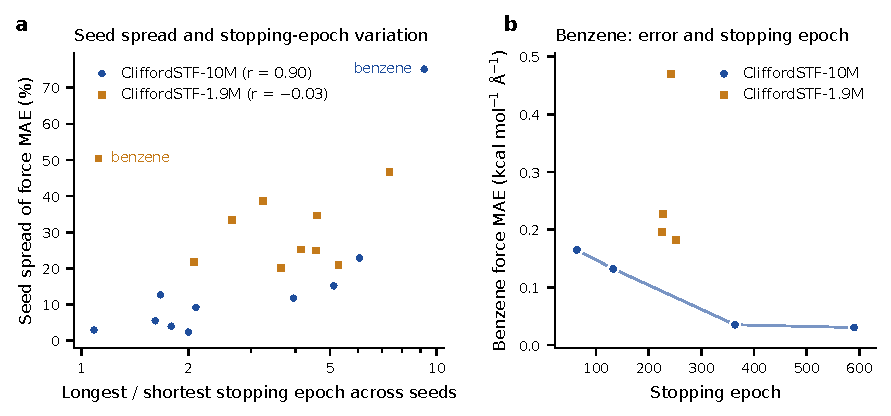
\includegraphics[width=0.92\textwidth]{figures/fig_seed.pdf}
\caption{\textbf{Seed spread and early stopping on rMD17.} (a) Relative standard deviation of test force MAE across four seeds against the ratio of the longest to shortest stopping epoch, one point per molecule ($n{=}10$ per configuration); $r$ is the Pearson correlation. (b) Benzene test force MAE against stopping epoch for each of the four seeds; the line joins the CliffordSTF-10M seeds in order of run length. Mean force cosine similarity exceeds $0.995$ for all 80 evaluations.}
\label{fig:seeds}
\end{figure}


\textbf{Memory.} Peak GPU memory on rMD17 aspirin (batch 32, 672 atoms and 11{,}456 edges per batch, RTX 4090, PyTorch 2.4.1) is $408$\,MiB at inference and $1{,}962$\,MiB in training for CliffordIP ($1.39\times10^6$ parameters), and $491$\,MiB and $2{,}596$\,MiB for CliffordSTF ($1.06\times10^6$ parameters): the dual-track scaffold costs $20\%$ more memory at inference and $32\%$ more in training at a slightly smaller parameter count.

\section{Wall-clock measurements at matched parameter budget}\label{supp:wallclock}

Table~\ref{tab:wallclock} reports rMD17 aspirin timings at approximately $10^6$ parameters, batch size 32, on a single GPU. Measurements use 10 warm-up steps followed by 20 timed steps. CliffordSTF takes $0.352$\,s per inference step and $7.77$\,s per training step, versus $0.128$ and $3.11$\,s for CliffordIP. Its inference time is comparable to ICTP $L{=}2/3$; training takes $1.25\times$ as long as ICTP $L{=}3$ and $3.13\times$ as long as EquiformerV2 $L{=}4$. The forward/backward decomposition is $2.59/5.10$\,s for CliffordSTF and $1.09/1.32$\,s for EquiformerV2 $L{=}4$, indicating a larger backward-pass cost in the dual-track implementation. These timings describe the measured implementations and hardware.

\begin{table}[!htbp]
\centering
\caption{\textbf{Wall-clock at matched parameter budget}, rMD17 aspirin, batch 32, single GPU. Time columns are mean $\pm$ standard deviation over 20 timed steps following 10 warmup steps; samples-per-second columns are derived from the means. Lower is faster for the time columns; higher is faster for the samples-per-second columns. All models fall within $\pm 50$\% of the $10^6$-parameter target. The Clifford and CliffordSTF (ours) entries reflect the optimized PyTorch dispatch described in Section~\ref{supp:optim}.}
\label{tab:wallclock}
\small
\begin{tabular}{lrrrrr}
\toprule
Model & Params & Train step (s) & Train (s/s) & Infer step (s) & Infer (s/s) \\
\midrule
PaiNN              & 1{,}043{,}856 & 0.79 $\pm$ 0.05 & 1{,}145 & 0.028 $\pm$ 0.003 & 3{,}575 \\
SchNet             &   984{,}769 & 1.16 $\pm$ 0.02 &   773 & 0.069 $\pm$ 0.011 & 1{,}456 \\
FAENet             & 1{,}027{,}745 & 1.69 $\pm$ 0.03 &   533 & 0.111 $\pm$ 0.004 &   900 \\
GotenNet           & 1{,}057{,}729 & 1.81 $\pm$ 0.00 &   497 & 0.064 $\pm$ 0.005 & 1{,}571 \\
MACE $L{=}1$       & 1{,}006{,}014 & 1.81 $\pm$ 0.29 &   497 & 0.160 $\pm$ 0.008 &   624 \\
EquiformerV2 $L{=}2$ &   891{,}560 & 2.45 $\pm$ 0.01 &   367 & 0.131 $\pm$ 0.001 &   764 \\
EquiformerV2 $L{=}3$ & 1{,}041{,}304 & 2.45 $\pm$ 0.01 &   367 & 0.135 $\pm$ 0.003 &   741 \\
EquiformerV2 $L{=}4$ & 1{,}043{,}222 & 2.48 $\pm$ 0.00 &   363 & 0.142 $\pm$ 0.008 &   702 \\
MACE $L{=}2$       & 1{,}011{,}683 & 2.53 $\pm$ 0.09 &   355 & 0.237 $\pm$ 0.002 &   422 \\
TorchMD-NET        &   968{,}242 & 2.58 $\pm$ 0.02 &   349 & 0.186 $\pm$ 0.029 &   538 \\
NequIP             & 1{,}002{,}436 & 3.06 $\pm$ 0.04 &   295 & 0.221 $\pm$ 0.007 &   452 \\
CliffordIP    & 1{,}031{,}926 & 3.11 $\pm$ 0.01 &   289 & 0.128 $\pm$ 0.000 &   781 \\
ViSNet             &   957{,}606 & 3.21 $\pm$ 0.07 &   280 & 0.235 $\pm$ 0.001 &   425 \\
MACE $L{=}3$       &   980{,}092 & 3.60 $\pm$ 0.16 &   250 & 0.261 $\pm$ 0.009 &   384 \\
ICTP $L{=}1$       & 1{,}039{,}554 & 4.50 $\pm$ 0.11 &   200 & 0.302 $\pm$ 0.052 &   331 \\
ICTP $L{=}2$       &   997{,}368 & 5.38 $\pm$ 0.10 &   167 & 0.364 $\pm$ 0.007 &   275 \\
DimeNet++          & 1{,}064{,}070 & 5.84 $\pm$ 0.11 &   154 & 0.326 $\pm$ 0.002 &   307 \\
ICTP $L{=}3$       &   982{,}752 & 6.23 $\pm$ 0.02 &   144 & 0.356 $\pm$ 0.006 &   281 \\
CliffordSTF (ours) & 1{,}056{,}534 & 7.77 $\pm$ 0.11 &   116 & 0.352 $\pm$ 0.001 &   284 \\
\bottomrule
\end{tabular}
\end{table}

\section{Implementation optimizations}\label{supp:optim}

The timings use standard PyTorch operations \citep{paszke2019pytorch} without custom CUDA or Triton kernels. The geometric product is evaluated by an \texttt{einsum} against a precomputed Cayley structure tensor. Graph counts are passed explicitly to avoid per-layer host synchronisation, layer-independent routing descriptors are computed once per forward pass, and validation metrics accumulate on device. Compilation is disabled in the reported configuration.

\section{Per-seed stability evidence for cross-track coupling}\label{supp:cross_stability}

We compare the existing \emph{Full} and \emph{Full no cross} runs using per-run errors, per-seed means and a count of unstable runs. The stored configurations show that \emph{Full no cross} disables both cross-track coupling and adaptive routing, so this comparison does not isolate coupling alone. Each configuration comprises 24 runs: 4 molecules (aspirin, benzene, ethanol, salicylic acid) $\times$ 6 seeds. The metric is test energy MAE in meV. The mean $\pm$ std reported in Table~\ref{M-tab:ablation} averages the four molecules within each seed and then takes mean and standard deviation over the six seeds; both levels of aggregation are given below.

The \emph{loss ratio} column normalises each run's final training loss by the median final training loss for that molecule across the twelve variants in the original \texttt{MD17\_Ablation} sheet, including the additional no-routing run series and excluding the later STF-only readout series, giving a molecule-independent scale on which a diverged optimisation is identifiable without reference to the test metric.

\begin{table}[!htbp]
\centering
\caption{\textbf{Per-run energy MAE and normalised final training loss}, Full versus Full no cross on rMD17. Loss ratio is the run's final training loss divided by the median final training loss for that molecule across the twelve original \texttt{MD17\_Ablation} variants. The single run with loss ratio above $5$ (aspirin, seed 4, no cross) is the only diverged optimisation in either configuration.}
\label{tab:cross_perrun}
\setlength{\tabcolsep}{6pt}
\begin{tabular}{llcccc}
\toprule
& & \multicolumn{2}{c}{\textbf{Full (cross on)}} & \multicolumn{2}{c}{\textbf{Full, no cross}} \\
\cmidrule(lr){3-4}\cmidrule(lr){5-6}
Molecule & Seed & $e_\mathrm{MAE}$ (meV) & Loss ratio & $e_\mathrm{MAE}$ (meV) & Loss ratio \\
\midrule
Aspirin & 1 & 51.74 & 0.52 & 24.08 & 0.45 \\
Aspirin & 2 & 11.55 & 1.11 & 42.16 & 0.71 \\
Aspirin & 3 & 69.21 & 0.66 & 57.93 & 2.80 \\
Aspirin & 4 & 7.93 & 1.11 & 963.07 & 25.24 \\
Aspirin & 5 & 12.01 & 3.09 & 24.42 & 1.78 \\
Aspirin & 6 & 72.88 & 2.45 & 17.21 & 0.88 \\
Benzene & 1 & 25.72 & 0.87 & 12.08 & 1.27 \\
Benzene & 2 & 24.35 & 2.05 & 61.82 & 2.31 \\
Benzene & 3 & 8.85 & 1.47 & 30.29 & 1.37 \\
Benzene & 4 & 30.75 & 0.77 & 32.89 & 1.45 \\
Benzene & 5 & 550.56 & 2.77 & 42.94 & 1.26 \\
Benzene & 6 & 6.96 & 0.47 & 46.87 & 2.28 \\
Ethanol & 1 & 3.04 & 0.86 & 7.58 & 0.93 \\
Ethanol & 2 & 32.70 & 4.71 & 16.70 & 0.92 \\
Ethanol & 3 & 2.86 & 0.54 & 14.22 & 1.09 \\
Ethanol & 4 & 14.00 & 0.83 & 11.96 & 0.60 \\
Ethanol & 5 & 12.31 & 0.54 & 33.78 & 1.32 \\
Ethanol & 6 & 12.52 & 0.87 & 13.60 & 0.99 \\
Salicylic & 1 & 29.71 & 0.56 & 74.36 & 1.27 \\
Salicylic & 2 & 38.07 & 0.51 & 56.54 & 1.10 \\
Salicylic & 3 & 54.69 & 0.81 & 29.86 & 0.71 \\
Salicylic & 4 & 21.60 & 0.70 & 23.34 & 1.01 \\
Salicylic & 5 & 4.29 & 1.09 & 10.11 & 1.18 \\
Salicylic & 6 & 5.36 & 0.95 & 42.01 & 1.62 \\
\bottomrule
\end{tabular}
\end{table}

\begin{table}[!htbp]
\centering
\caption{\textbf{Seed-level energy MAE} (molecule-averaged, the aggregation used in Table~\ref{M-tab:ablation}) and summary statistics at both aggregation levels.}
\label{tab:cross_summary}
\setlength{\tabcolsep}{6pt}
\begin{tabular}{lcc}
\toprule
& \textbf{Full (cross on)} & \textbf{Full, no cross} \\
\midrule
\multicolumn{3}{l}{\emph{Seed-level $e_\mathrm{MAE}$ (meV), molecules averaged within seed}} \\
1 & 27.55 & 29.52 \\
2 & 26.67 & 44.30 \\
3 & 33.90 & 33.08 \\
4 & 18.57 & 257.81 \\
5 & 144.79 & 27.81 \\
6 & 24.43 & 29.92 \\
\midrule
Seed-level median   & 27.11 & 31.50 \\
Seed-level mean $\pm$ std & 45.99 $\pm$ 48.66 & 70.41 $\pm$ 92.00 \\
\midrule
\multicolumn{3}{l}{\emph{Run-level statistics (all 24 runs)}} \\
Median $e_\mathrm{MAE}$ (meV)      & 17.80 & 30.07 \\
Interquartile range (meV)          & 8.6--34.0 & 16.1--43.9 \\
Maximum $e_\mathrm{MAE}$ (meV)     & 550.56 & 963.07 \\
Runs with $e_\mathrm{MAE} > 50$\,meV   & 5/24 & 5/24 \\
Runs with $e_\mathrm{MAE} > 100$\,meV  & 1/24 & 1/24 \\
Runs with loss ratio $> 5$         & \textbf{0/24} & \textbf{1/24} \\
Mean $\pm$ std excluding worst run (meV) & 24.05 $\pm$ 20.86 & 31.60 $\pm$ 18.69 \\
Median $f_\mathrm{cos}$            & 0.547 & 0.490 \\
\bottomrule
\end{tabular}
\end{table}

\FloatBarrier

\textbf{Summary.} In the full STF$_2$+STF$_3$ configuration, the observed divergence count is 0/24 runs with coupling and 1/24 without it, unchanged at loss-ratio thresholds of 5, 10 and 20. Median run-level energy MAE is $17.8$ versus $30.1$\,meV, with coupling lower in 16 of 24 matched molecule--seed pairs. The paired differences are not statistically significant at this sample size (Wilcoxon signed-rank test \citep{wilcoxon1945ranking}: $p=0.229$ for energy MAE and $p=0.623$ for force cosine). The two configurations each contain one large test-energy outlier; the coupled benzene outlier has a loss ratio of $2.77$ and is not classified as a training divergence. Divergence is therefore defined from training loss rather than test energy error.

The result is configuration-dependent. Removing coupling from the STF$_2$-only model improves mean energy MAE from $34.9$ to $25.8$\,meV and force cosine from $0.421$ to $0.456$.
